\input{header}

\AtBeginSubsection[]
{
	\begin{frame}<beamer>
		\frametitle{Outline}
		\tableofcontents[current,currentsubsection]
	\end{frame}
}

\begin{document}

\begin{frame}[allowframebreaks] \frametitle{Reductions via Computation Histories}
\begin{itemize}
\item This is a technique to prove that $A_{\text{TM}}$ is reducible to
  some languages
\item Thus it can be used to prove that a language is undecidable
\item We will show that the method is useful when the
  undecidable language involves testing for the
  existence of something (or say checking if a language
  is empty)
\item For example, it is used to prove the undecidability of
  Hilbert's 10th problem, testing for the existence of integral roots
  in a polynomial (details not shown)
\item What is the computation history of a TM?
\item It is the sequence of configurations the machine goes
  through
\item Formal definition: $M$ a TM and $w$ an input string
\item [] An accepting computation history for $M$ and $w$ is
  \begin{equation*}
    C_1, \ldots, C_l,
  \end{equation*}
where
\begin{center}
  \begin{tabular}{l}
    $C_1$  is the start configuration,\\
    $C_l$ is an accepting configuration, and\\
    $C_i$ follows from $C_{i-1}$
  \end{tabular}
\end{center}
\item A rejecting computation history is similar,
  except that $C_l$ is a rejecting configuration
\item Computation histories are finite sequences
\item[] If $M$ does not halt on $w$, no accepting or
  rejecting computation history for $M$ on $w$
\item Deterministic TM has at most one history on an input
\item [] It may have zero if a loop occurs
\item NTM may have many histories
  \end{itemize}\end{frame}
\begin{frame}[allowframebreaks] \frametitle{Linear Bounded Automaton (LBA)}
  \begin{itemize}
  \item We will use computation histories to show some related
    problems of LBA are undecidable
  \item A linear bounded automaton (LBA) is
    a special TM:
head cannot move beyond the end of input
\item If the head tries to move right at the end
  of input, the head stays
\item It is similar to moving left at the beginning of the
  tape
\item Therefore, we have
  \begin{center}
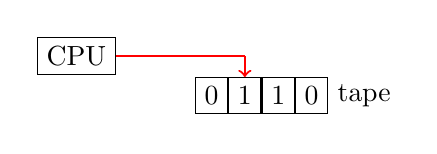
\begin{tikzpicture}[ampersand replacement=\&]
\matrix 
{
  \node[draw](0) {CPU}; \& [1cm] \& \node(1){}; \&\&\& \\
  \& \node[draw]{0}; \& \node[draw](a){1}; \& \node[draw]{1}; \& \node[draw]{0};  \& \node{tape};\\
};
\draw [-,red,thick] (0) -- (1.center) ;
\draw [->,red,thick] (1.center) -- (a) ;
\end{tikzpicture}
\end{center}
  
\item An LBA is a TM with limited memory: the tape length is $n$, the input length
\item This ``limited memory'' description seems to be strange as $n$ is not a constant
\item Let's use another (equivalent) way to define LBA
  as follows\footnote{Descriptions come from \url{https://en.wikipedia.org/wiki/Linear_bounded_automaton}}
  \begin{enumerate}
  \item $\Gamma$ includes 2 special symbols: left and right
    end markers
  \item For any input, let's have markers in the beginning and in
    the end
  \item Transitions may not print other symbols over the endmarkers
  \item Transitions may neither move to the left of the left endmarker nor to the right of the right endmarker.
  \end{enumerate}
\item Then we still have a tape of infinite length, but impose
  restricted operations
\item Despite memory or operation constraints, LBAs are quite powerful
\item $A_{\text{DFA}}$, $A_{\text{CFG}}$, $E_{\text{DFA}}$, $E_{\text{CFG}}$
  are all LBAs (details not discussed)
\end{itemize}\end{frame} 

\begin{frame}[allowframebreaks]
\frametitle{LBA's \# of Configurations}
\begin{itemize}
\item We prove that an LBA has a finite number of
  configurations
\item For an LBA $M$, if
  \begin{center}
    \begin{tabular}{l}
      $q$: \# states = $|Q|$,\\
      $g$: \# symbols = $|\Gamma|$,
    \end{tabular}
  \end{center}
  then $M$ has exactly $qng^n$ distinct
  configurations for a tape of length $n$
\item Proof: a configuration involves
  \begin{center}
    current state, head position, tape contents
  \end{center}
  \item
    Immediately we see
    \begin{equation*}
      q \qquad n \qquad g^n
    \end{equation*}
    possibilities for each
  \item Thus the total number of possibilities is $qng^n$
\end{itemize}
\end{frame}

\begin{frame}[allowframebreaks]
\frametitle{$A_{\text{LBA}}$ Decidable}
\begin{itemize}
\item Consider
  \begin{equation*}
  A_{\text{LBA}}=
\{\langle  M,w\rangle\mid M \mbox{ is an LBA that accepts } w\}
\end{equation*}
  \item In applying $M$ on $w$, the concern is that $M$
    loops on $w$
  \item Now tape length is fixed to $|w|=n$ (or say we will never
    use more than $n$ positions)
  \item If a loop occurs, one configuration 
appears twice
\item Thus we check if in $qng^n$ steps, same configurations occur
\item This is a finite procedure so $A_{\text{LBA}}$ is
  decidable
\end{itemize}
\end{frame}

\end{document}

%%% Local Variables:
%%% mode: latex
%%% TeX-master: t
%%% End:
